\documentclass[11pt]{scrartcl}
\usepackage{dominatrix}

\usepackage{listings}
\lstset{language=Awk}
\lstset{frame=single}
\lstset{framesep=10pt}
\lstset{upquote=true}
\lstset{basicstyle=\ttfamily}

\lstset{emph={awk}, emphstyle=\textbf}

\usepackage{colortbl}
\usepackage{pgfplots}
\newcommand{\jon}{Jón }
\newcommand{\ve}{\varepsilon}
\pgfplotsset{compat=1.9}
\renewcommand\thesubsection{\alph{subsection}}
\definecolor{light-gray}{gray}{0.75}
\title{Household Behavior}
\subject{ECON W3213 Spring 2014 \jon Steinsson}
\author{Linan Qiu, lq2137}
\begin{document}
\maketitle

\begin{abstract}
This set of recitation notes covers \textbf{Household Behavior} (sometimes referred to as labor leisure decisions). This is in no way a substitute for attending lectures, but just in case you dozed off or checked your boyfriend's Facebook page while \jon was working Calculus magic on the board, this set of notes should save you.

Also, I occasionally spell behavior as behaviour. Pardon me. A relic of my post-colonial education in Singapore.
\end{abstract}

\section{Household Utility}

First, we assume that 

\begin{itemize}
	\item You \textbf{love consuming}. I don't just mean eating (though that comes really close). I mean all sorts of hedonistic luxuries and necessary necessities that you shower on yourself. 
	\item You \textbf{hate working}. I had a hard time coming to terms with this, since I kind of enjoy doing these recitation notes, but then I remembered my time working as a conscript in the army. Phew.
\end{itemize}

In that case, whatever you consume should increase your utility, and however much you work should decrease your utility. Hence, \textbf{overall utility} is

\[ U(C) - V(H)\]

Where 
\begin{itemize}
	\item $U(C)$ represents utility from consumption of goods
	\item $V(H)$ represents disutility (ie. pain) from working (ie. supplying labor)
\end{itemize}

Of course, we realize that the number of hours worked \emph{per person} $H$ is equal to the total labor supply $L$ divided by the number of people $N$. Hence

\[L = NH\]

Most of the time, we simply normalize $N = 1$. This doesn't mean there's only one person in our population -- for all we care $N$ can be in the billions. However, modifying $N$ doesn't really add much meaning to our model but adds way too much complexity in calculations, so we simply "normalize" it to 1. 

\section{Properties of the Household Utility Function}

We demand that the household utility function should have the following properties

\subsection{Utility Increases as Consumption Increases}
If you eat more cookies, you get happy. That's an universal law. Mathematically, we say

\[ \frac{\partial U(C)}{\partial C)} = U'(C) > 0\]

Just a reminder: $U'(C)$ is simply a shorthand for the first order derivative of $U$ with respect to $C$. 

\subsection{Marginal Utility of Consumption Decreases}
If I keep stuffing you with cookies, you'll get sick of it. That is, you get less utility per additional cookie. Mathematically, we say

\[ \frac{\partial^2 U(C)}{\partial C^2} = U''(C) < 0\]

Just a reminder: $U''(C)$ is simply a shorthand for the second order derivative of $U$ with respect to $C$. 

\subsection{Utility Decreases as Work Increases}
If $V(H)$ represents pain one gets from working, then the more you work, the more pain you get right? Mathematically, we represent this as

\[ \frac{\partial V(H)}{\partial H} = V'(H) > 0\]

Note that $V(H)$ \textbf{increases} as $H$ increases, but that leads to overall utility \textbf{decreasing} because of the \textbf{negative sign} in front of $V(H)$.

\subsection{Marginal Disutility of Working Increases}
If I hole you up in a factory and make you work for 12 hours, the \nth{13} hour will be intolerable -- way more so than the \nth{1} hour. Hence your pain increases at an increasing rate. Mathematically, we say

\[\frac{\partial^2 V(H)}{\partial H^2} = V''(H) > 0\]

\subsection{Graphical Representations}

The 4 conditions above naturally causes the plots of $U(C)$ and $V(H)$ to look like these. 

\begin{figure}[ht!]
\begin{subfigure}[b]{0.5\textwidth}
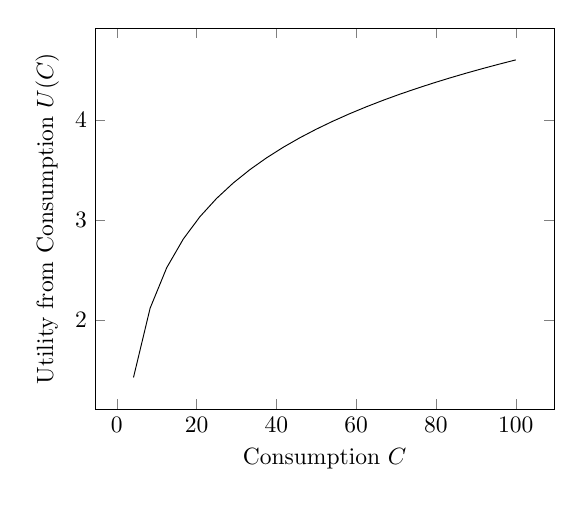
\begin{tikzpicture}[scale=0.85]
\begin{axis}[xlabel={Consumption $C$},ylabel={Utility from Consumption $U(C)$}]
\addplot[domain=0:100,black]
{(ln(x))};
\end{axis}
\end{tikzpicture}
\caption{Plot of $U(C)$ against $C$}
\end{subfigure}
\hspace{2ex}
\begin{subfigure}[b]{0.5\textwidth}
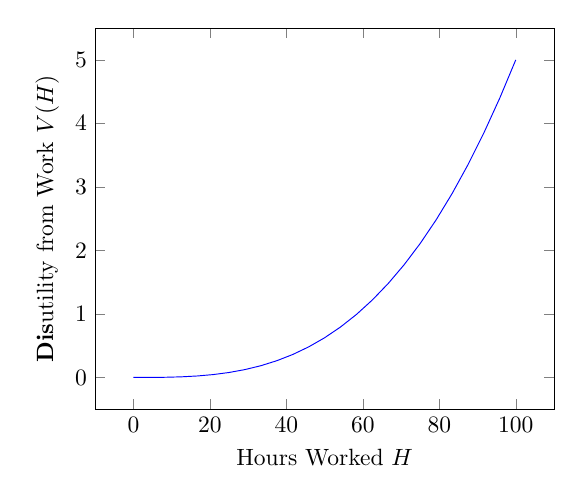
\begin{tikzpicture}[scale=0.85]
\begin{axis}[xlabel={Hours Worked $H$},ylabel={\textbf{Dis}utility from Work $V(H)$}]
\addplot[domain=0:100,blue]
{(x^(3)/(200000))};
\end{axis}s
\end{tikzpicture}
\caption{Plot of $V(H)$ against $H$}
\end{subfigure}
\caption{Plots of $U(C)$ and $V(H)$}
\end{figure}

Again, you like eating cookies, so you get happier as you eat them. But each additional cookie brings you less happiness. Substitute cookie for your choice of poison.

You hate working. At first, you simply hate the job. After a 24 hour shift, you start hating the whole world. Just imagine your least favorite job in the world.

\section{Labor Supply}

\subsection{Labor Supply by Optimization}
After we have the utility function, all that's left to do is to find the maximum utility. In other words, we are optimizing it.

But before we optimize, we know that there's a \textbf{budget constraint} that we have to obey: you can't spend more than you earn. In other words, $C = wH$. Pretty self-evident.

Hence, we are trying to

\[\max U(C) - V(H) \]
\[\mathrm{st.} C=wH\]

We substitute the constraint into the utility function, turning it into

\[U(wH) - V(H)\]

Now we ask, "How much should I work, given a certain wage, to maximize my utility?"

That is equivalent to doing

\begin{align*}
\frac{\partial [U(wH) - V(H)]}{\partial H} &= \frac{\partial U(wH)}{\partial H} - \frac{\partial V(H)}{\partial H} \\
&= wU'(wH) - V'(H) = 0 \\
\end{align*}

With some algebra magic, we arrive at

\[ \frac{V'(H)}{U'(wH)} = \frac{V'(H)}{U'(C)} = w \]

This is the \textbf{Labor Supply Equation}. The fact that we arrive at the labor supply equation shouldn't surprise us at all. After all, we were asking the question: how much labor should one provide in order to maximize one's utility? What we have just derived is then the condition that dictates how one should supply his labor, hence the labor supply equation!

\subsection{Labor Supply by Calculus of Variations}

There's another way to derive the optimum labor supply. 

First, let's assume that we are at the optimum labor supply $H=H^*$ That means we're already bloody happy. There's no way to make us happier by working less or more. 

We can express our current utility as

\[U(wH^*) - V(H^*)\]

Now let's say I work just a \emph{little} more by $\ve$ hours. In that case, my utility will be 

\[U(w(H^*+\ve)) - V(H^*+\ve)\]

Remember \textbf{Taylor Series Approximation}? If you don't, go reread the set of notes titled \lstinline{00 Mathematics Crash Course.pdf}. I actually used this exact example!

We know that this can be approximated by

\[ U(w(H^*+\ve)) - V(H^*+\ve) = U(wH^*) - V(H^*) + [wU'(wH^*) - V'(H^*)]\ve + e \]

Where $e$ simply represents the error in approximation.

Since we know that $H^*$ was already optimum, then whatever utility that results from moving away from $H^*$ must be less than or equal to the utility at $H*$. Hence,

\[ U(w(H^*+\ve)) - V(H^*+\ve) \leq U(wH^*) - V(H^*) \]

Let's explore this inequality further. The approximation tells us that

\begin{align*}
U(w(H^*+\ve)) - V(H^*+\ve) - U(wH^*) - V(H^*) &= [wU'(wH^*) - V'(H^*)]\ve + e \\
&\leq 0
\end{align*}

We know that the smaller our approximation is, the smaller $e$ is. This goes to the point that the limit of $e$ as $\ve$ tends to $0$ is $0$. So let's just treat $e$ as zero.

Then,

\[ [wU'(wH^*) - V'(H^*)]\ve \leq 0 \]

In order for this inequality to be true for all $\ve$, $wU'(wH^*) - V'(H^*) = 0$.

\begin{align*}
wU'(wH^*) - V'(H^*) &= 0 \\
wU'(wH^*) &= V'(H^*) \\
\frac{V'(H^*)}{U'(wH^*)} &= \frac{V'(H^*)}{U'(C^*)} = w
\end{align*}

We arrive at the exact same conclusion. This is just a fancier way to do it. Now go impress your date. \textbf{Actually, please don't.}

\subsection{Labor Supply by Pure Intuition}
After we have gone through a simple method (by simple optimization), a tough as hell method (by calculus of variations), let's try something even simpler -- \textbf{intuition}.

Suppose that you're already at optimum, that is $H = H^*$. You'd want the marginal benefit of working to be equal to the marginal cost of working. You don't need me to explain why that's the case right?

\begin{itemize}
	\item The marginal benefit of working an additional $\ve$ hour is $\ve U'(C^*) = \ve  w  U'(wH^*)$ It is the number of hours worked $\ve$ times the marginal benefit per hour worked. 
	\item The marginal cost of working an additional $\ve$ hours is $\ve V'(H^*)$, since $V'(H^*)$ is the disutility (hence marginal cost) of working one additional hour.
\end{itemize}

\begin{align*}
wU'(C^*) &= V'(H^*) \\
\frac{V'(H^*)}{U'(C^*)} &= w
\end{align*}

Voila!

These 3 methods are essentially saying the same thing. And they naturally arrive at the same result.

\subsection{Labor Demand}

What about \textbf{Labor Demand Equation}? Well, we already derived that in the previous set of notes \lstinline{01 Production.pdf}. To recall, we maximized the profits of the firm by 

\begin{align*}
\max \pi &= \max (Y - wL - rK) \\
&= \max (\bar{A}K^\alpha L^{1-\alpha} - wL - rK \\
&= \bar{A} K^\alpha (1-\alpha)L^{-\alpha} - w = 0
\end{align*}

\[ w = \bar{A}K^\alpha (1-\alpha)L^{-\alpha} = (1-\alpha) \frac{Y}{L}\]

By equating these two equations, we can find the optimum labor supply (since we know that $L = NH$). After knowing the optimum $H$ or $L$ (it doesn't really make a difference, since we can find one from the other given $N$. Now you know why I normalized $N=1$ for convenience?), we can find the equilibrium wage $w$ too.

\subsection{Slope of Labor Supply}
The next question to ask is: what if I change wage $w$? How will the amount of labor supplied change? Eventually, how does my labor supply curve look like.

To understand this, we need to know that two things happens when wage changes.

\begin{itemize}
	\item \textbf{Substitution Effect} happens when wage changes. Say wage increases. Leisure is more "expensive" relative to goods since wage is the opportunity cost of leisure. Then, we will work more. Hence, we "substitute" leisure with work due to the change in "price" of leisure.
	\item \textbf{Income Effect} happens when wage changes too. Say we have higher wages. We are now richer. Then we afford to consume more AND enjoy more time off. 
\end{itemize}

\begin{table}[ht!]
\begin{longtable}{c|cc}
\hline
Wages & Increase & Decrease \\
\hline
Substitution Effect & Work More & Work Less \\
Income Effect & Work Less & Work More \\
\hline
\end{longtable}
\caption{Substitution and Income Effects}
\end{table}

The overall effects from wage changes are kind of dubious. So let's investigate further.

\subsubsection{Substitution Effect}
When we look at the substitution effect, we want to consider the effects of varying the wage \textbf{without changing consumption}. 

\[\frac{V'(H)}{U'(C)} = w\]

So we hold $C$, therefore $U'(C)$ constant.

Then, if I increase $w$, what happens to the labor supply equation? Naturally, on the left, $V'(H)$ must increase as well to maintain the equality. 

This is the tricky part. We are increasing $V'(H)$ not $V(H)$, so we are asking how do we increase the \textbf{slope} of $V(H)$, not the value of $V(H)$ itself. Let's bring back the plot of $V(H)$.

\begin{figure}[ht!]
\centering
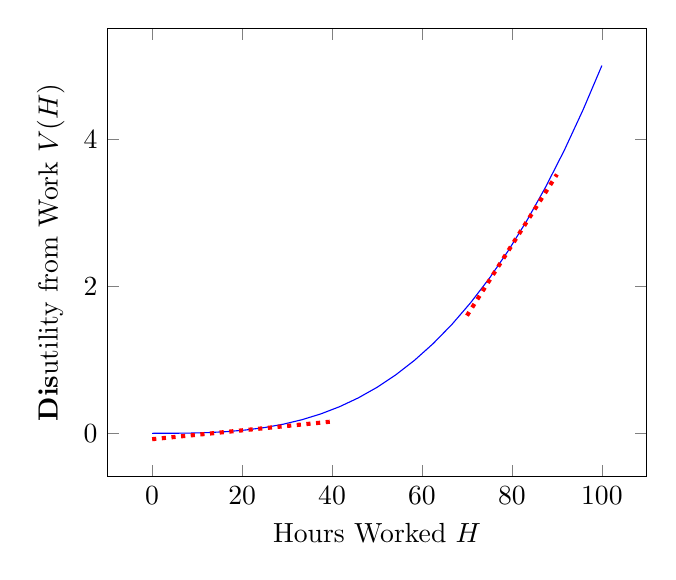
\begin{tikzpicture}
\begin{axis}[xlabel={Hours Worked $H$},ylabel={\textbf{Dis}utility from Work $V(H)$}]
\addplot[domain=0:100,blue]
{(x^(3)/(200000))};
\addplot[domain=0:40,red,dotted, line width = 1.5]
{(0.006*x-0.08)};
\addplot[domain=70:90,red,dotted, line width = 1.5]
{(0.096*x-5.12)};
\end{axis}s
\end{tikzpicture}
\caption{Plot of $V(H)$ against $H$}
\end{figure}

If I want to increase $V'(H)$ (which is the slope of the tangent as drawn in the plot), I probably want to move to a higher $H$.

Technically, this is because $V(H)$ is concave, hence $V''(H) > 0$, hence when we want increase $H$, $V'(H)$ increases. Remember, $V''(H)$ describes how $V'(H)$ will change when $H$ changes.

Does this fit in with our intuition? Surely it must. When wages increase, people slack off less because slacking off becomes more expensive. So they choose less leisure and work more instead.

Try working out the case where $w$ decreases!

\subsubsection{Income Effect}
When we look at the income effect, we want to consider the effects of varying consumption $C$ \textbf{without changing wages}. I know we talked about changing wages earlier, so follow this logic.

\begin{enumerate}
	\item Imagine that wages increases.
	\item The substitution effect shows the effect of wage changing without consumption changing. 
	\item Then we investigate what happens when consumption changes, holding wages constant.
	\item This gives us all the effects of wages increasing.
\end{enumerate}

\[\frac{V'(H)}{U'(C)} = w\]

If $C$ increases, what happens to this equation? Let's look at what happens to $U'(C)$ first.

\begin{figure}[ht!]
\centering
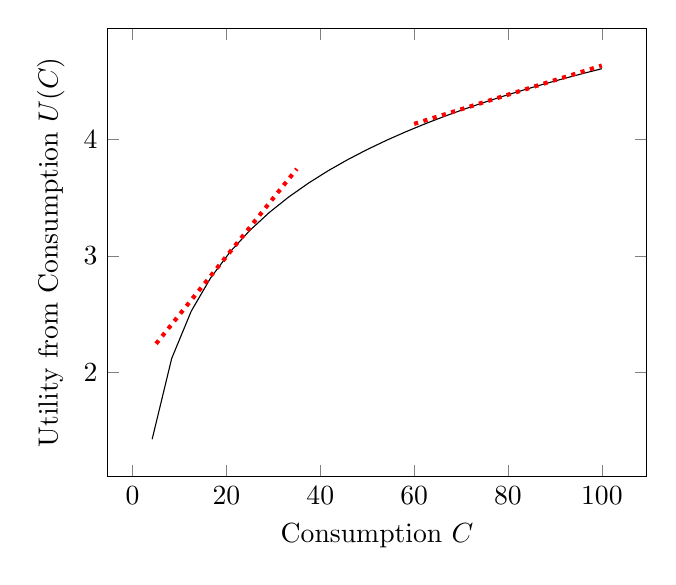
\begin{tikzpicture}
\begin{axis}[xlabel={Consumption $C$},ylabel={Utility from Consumption $U(C)$}]
\addplot[domain=0:100,black]
{(ln(x))};
\addplot[domain=5:35,red,dotted, line width = 1.5]
{(0.05*x+1.9957)};
\addplot[domain=60:100,red,dotted, line width = 1.5]
{(0.0125*x+3.382)};
\end{axis}
\end{tikzpicture}
\caption{Plot of $U(C)$ against $C$}
\end{figure}

If $C$ increases, $U'(C)$ decreases. Again, this is because $U''(C) < 0$.

Then for the equality to hold, $V'(H)$ must decrease. That means $H$ must decrease.

Again this fits in with intuition -- when we are richer, we simply work less.

\subsubsection{Comparison of Effects}

\begin{table}[ht!]
\begin{longtable}{c|cc}
\hline
Wages & Increase & Decrease \\
\hline
Substitution Effect & Work More & Work Less \\
Income Effect & Work Less & Work More \\
\hline
\end{longtable}
\caption{Substitution and Income Effects}
\end{table}

Evidently, these two effects affect labor supply in opposite directions. The overall change in labor supply depends on the extent of changes in wages.

\begin{itemize}
	\item If wage change occurs only in the \textbf{short run} (for example, due to a government recession subsidy program), then you know that you will end up getting poorer later on. So you may not spend a lot more. Income effect is small, and \textbf{substitution effect} dominates.
	\item If wage change is in the \textbf{long run}, then you know that you'll be richer permanently. Historically, these two effects then \textbf{cancel out}. 
\end{itemize}

\section{Taxation}

\subsection{Taxation, Budget Constraint, and Optimization}

Let's throw 3 more things into our model

\begin{itemize}
	\item Income Tax $\tau_l$
	\item Consumption Tax $\tau_c$
	\item Government Transfers $T$
\end{itemize}

Your utility function still remains the same as 

\[ U(C) - V(H) \]

After all, your preferences don't change just because of taxation. However, your budget constraint changes to

\[(1+\tau_c)C = (1-\tau_l)wH + T\]

On the left side, your spendings are augmented by the consumption tax. On the left side, your income is is reduced by the amount of the taxation. Additionally, if the government decides to throw some of your tax money back at you (in the form of say education, medical subsidies etc), then that transfer adds on to your income.

Remember that without taxes, 

\[\frac{V'(H)}{U'(C)} = w = (1-\alpha)\frac{Y}{L}\]

That's \textbf{labor supply equals labor demand}.

With taxes however, you'll find that the labor supply becomes

\begin{align*}
\max [U(C) - V(H)] &= \max \left[U\left(\frac{(1-\tau_l)wH}{(1+\tau_c)} + \frac{T}{(1+\tau_c)} \right) - V(H)\right] \\
&= \left[\frac{(1-\tau_l)w}{(1+\tau_c)} * U'\left(\frac{(1-\tau_l)wH}{(1+\tau_c)} + \frac{T}{(1+\tau_c)} \right) - V'(H) \right] \\
&= \frac{(1-\tau_l)w}{(1+\tau_c)}U'(C) - V'(H) = 0
\end{align*}

\[\frac{V'(H)}{U'(C)} = w \frac{1-\tau_l}{1+\tau_c} < w\]

Post-tax wage is less than pre-tax wage.

\subsection{Taxation and Labor Supply}
So what happens to labor supply after taxation? Now we remember that there are two effects -- \textbf{income} and \textbf{substitution} effects. 

The magnitude of the \textbf{income effect} depends on what the government does with the tax revenue. Suppose the government taxes you \$1,000, but returns all the money back to you as cookies. Do you feel poorer? Not really! Because you were going to use that money to buy cookies anyway. Now replace cookies with healthcare and education. That works too right? So \textbf{income effect will be zero if government completely rebates taxes in the form of transfers}.

But what if the government took all that money, and used it to fund a war? Or worse still, use it to hold a giant Justin Bieber concert that no one goes to? Then you'd feel a lot poorer (barring any externalities from listening to Bieber). \textbf{Income effect will be large if the government does not rebate taxes}.

Let's assume that the \textbf{government DOES rebate all the money as lump sum transfers back to you}. That means if you paid \$1,000 in taxes, the government literally gives you a handout of \$1,000. This means that the \textbf{income effect is zero}.

Let's give a specific form to our utility function.

\begin{align*}
U(C) &= \log{C} \\
V(H) &= \psi \frac{H^{1+\eta}}{1+\eta}
\end{align*}

There's really nothing special about these functions, other than the fact that they obey the \emph{four conditions} we require of our utility function.

The overall utility function is then

\[\log{C} - \psi \frac{H^{1+\eta}}{1+\eta}\]

\begin{align*}
U'(C) &= \frac{1}{C} \\
V'(H) &= \psi H^\eta \\
\frac{V'(H)}{U'(C)} &= \psi H^\eta C = w \frac{1-\tau_l}{1+\tau_c}
\end{align*}

This is \textbf{Labor Supply}.

We remember that \textbf{Labor Demand} is

\[ w = (1-\alpha)\frac{Y}{L}\]

Combining (hence equilibrating)

\[ \psi H^\eta C = (1-\alpha)\frac{Y}{L} \left(\frac{1-\tau_l}{1+\tau_c}\right) \]

Remember that $L=NH$? Also, since we're assuming that the government transfer all taxes back as rebates, $C = \frac{Y}{N}$. Plugging these conditions in, we get

\[ \psi H^\eta C = (1-\alpha)\frac{C}{H} \left(\frac{1-\tau_l}{1+\tau_c}\right) \]

Rearranging in terms of $H$, we get

\[H^{\eta+1} = \left(\frac{1+\tau_c}{1-\tau_l}\right)^{-1} \frac{1-\alpha}{\psi}\]

Taking log, we get

\begin{align*}
\log{H^{\eta+1}} &= \log{\left(\frac{1+\tau_c}{1-\tau_l}\right)^{-1}} + \log{\frac{1-\alpha}{\psi}} \\
(\eta +1) \log{H} &= -\log{\left(\frac{1+\tau_c}{1-\tau_l}\right)} + \log{\frac{1-\alpha}{\psi}} \\
\log{H} &= -\frac{1}{\eta+1}\log{\left(\frac{1+\tau_c}{1-\tau_l}\right)} + \frac{1}{\eta+1}\log{\frac{1-\alpha}{\psi}}
\end{align*}

This means that a 1\% change in $\frac{1+\tau_c}{1-\tau_l}$ will lead to a $\frac{1}{\eta+1}$\% change in hours. 

Obviously $\eta$ is important, so important that we give it a name -- $\frac{1}{\eta}$ is known as the Frisch elasticity of labor supply.


\end{document}